\def\currentRootFolder{chapter/sensitivityStudyWithPreliminaryKatrinElossModel}
\def\currentFigureFolder{\currentRootFolder/fig}

\chapter{Parameter Inference Using an Energy Loss Model for Inelastically-Scattering Electrons Derived from KATRIN Data}
\label{sec:katrinEloss}
A quantitative accurate description of the scattering processes of $\upbeta$ electrons within KATRIN's gaseous tritium source is of crucial importance for the neutrino-mass-sensitivity goal. In modeling the corresponding effects the energy loss function as described in section~\ref{sec:intSpecModelResponseEloss}) plays an important role. With reference to the described energy loss function, the KATRIN Design report states, that its precision is not sufficient for the KATRIN-sensitivity goal. It was planned to deduce a sufficiently accurate model from data taken at KATRIN~\cite{Angrik:2005ep}. Such a model has successfully been established preliminarily for electrons scattering from deuterium molecules based on data taken in October 2018 by a dedicated subgroup of the KATRIN collaboration. This new energy loss model, from here forth named ``the KATRIN model'', has improved uncertainties with respect to the model from literature (section~\ref{sec:intSpecModelResponseEloss}), from here forth named ``the Aseev model'' after the primary author of the corresponding publication~\cite{Aseev2000}. Within the scope of this thesis the impact on KATRIN's sensitivity by the exchange of the Aseev model for the KATRIN model was studied. Therefore, this chapter is structured as follows: Section~\ref{sec:katrinElossConcept} presents the general idea of this study. Section~\ref{sec:katrinElossModel} outlines the KATRIN model. Section~\ref{sec:katrinElossStatistics} introduces the necessary statistical tools. Section~\ref{sec:katrinElossModelResults} lists and discusses the results. And section~\ref{sec:katrinElossModelConclusion} concludes and offers an outlook.

\section{Introduction and Motivation}
\label{sec:katrinElossConcept}
For the conducted sensitivity study KATRIN-neutrino-mass measurements were simulated assuming a neutrino mass of \SI{0}{eV} and using the KATRIN energy loss model. An uncertainty interval was deduced using the profile likelihood method as described in a subsequent section~\ref{sec:katrinElossStatistics} \todo{proper section}. This enables the treatment of the model uncertainties and their correlations as nuisance parameters.

It should be noted, that the KATRIN model used in this thesis is still preliminary and may be subject to changes. In fact, by the time of writing this thesis it has already undergone small adaptions to the version used in this chapter. However the form of the model has stayed the same, only the parameter values changed slightly. The newer and older parameter set are printed side by side in the appendix~\ref{sec:}. \todo{appendix}.

Furthermore, during a neutrino mass measurement, the nominal tritium purity in the~\gls{wgts} is~\SI{95}{\percent}. Here, an energy loss model for deuterium is used. Two different, but similar energy loss models are expected for the two different gas species (compare~\cite{Abdurashitov2017} and~\cite{Aseev2000}). Within the scope of this thesis, the impact on KATRIN's sensitivity from the reduction of uncertainties on the energy loss model are of primary interest. As long as the KATRIN model for deuterium is sufficiently similar to the model for tritium, it is a plausible approach to use it for simulations of KATRIN-neutrino-mass measurements. (For the similarity, see figure~\ref{fig:katrinElossElossModel}.) In that regard, the results for KATRIN's sensitivity derived in this chapter are expected to be meaningful.

Moreover, it is of interest to implement the required statistical tools into the available software frameworks in order for the study to be repeated or extended if needed. This will most likely be the case, when data for scattering from tritium are evaluated. Additionally, the approach taken in the scope of this thesis is explained in a general manner and may be applied to other model uncertainties, not only the once stemming from the energy loss function.

\section{The Preliminary KATRIN Energy Loss Model}
\label{sec:katrinElossModel}
\begin{figure}[tbh]
	\centering
	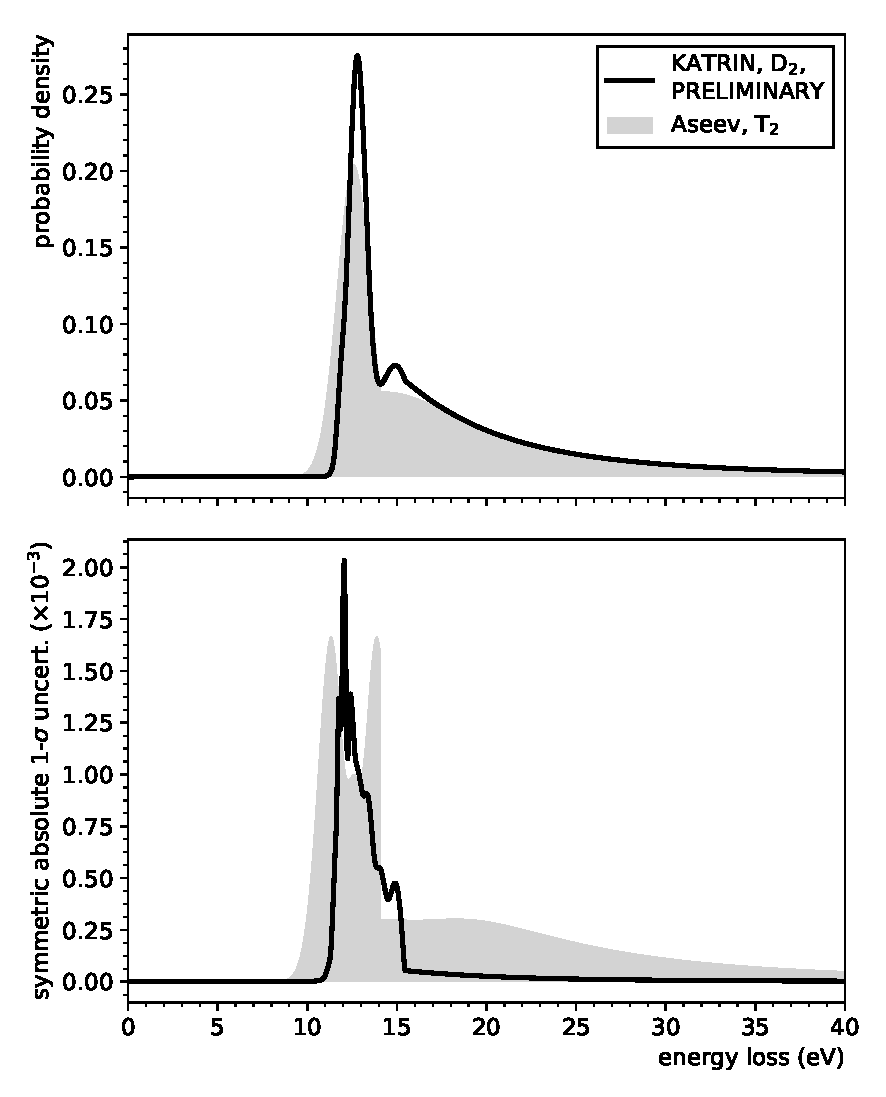
\includegraphics[width=\textwidth]{\currentFigureFolder/KATRINandAseevElossModel}
	\xcaption{The preliminary model for the energy loss of electrons scattering from deuterium molecules established at KATRIN}{The preliminary model for the energy loss of electrons scattering from deuterium molecules established at KATRIN.}{}
	\label{fig:katrinElossElossModel}
\end{figure}
The presented KATIRIN energy loss model is a phenomenological description fitted to data taken at the KATRIN experiment in October 2018. It was established by a dedicated subgroup of the KATRIN collaboration. As the model is still in its early stages this work refrains from a detailed physical interpretation and instead focuses on its statistical features. For the physics behind the model the reader is referred to the KATRIN documents specified in the footnote \footnote{\url{fuzzy.fzk.de/bscw/bscw.cgi/1254307}}\footnote{\url{neutrino.ikp.kit.edu/katrin/images/b/bf/D2_eloss_parametrization_v2.pdf}}\footnote{\url{nuserv.uni-muenster.de:8443/afulst/KATRIN-eloss/}}. Figure~\ref{fig:katrinElossElossModel} shows the KATRIN model in comparison to the Aseev model. Both match well in their general form and especially in the ionization tail.

With respect to the statistical properties, the KATRIN model shows an improved uncertainty in the ionization tail and also in large parts of the excitation peak.

The KATRIN model is based on the sum of three scaled Gaussian distributions to model the excitation peak region and an ab initio description for the ionization tail seamlessly attached to the model of the excitation peak region. The whole model can be described by 9 parameters which comprise the scales $A_i$, means $m_i$ and standard deviations $s_i$ of the three Gaussian distributions
\begin{equation}
	\nuisanceParamVec_\mathrm{eloss} = 
	\transp{\left(
	A_1, m_1, s_1, 
	A_2, m_2, s_2, 
	A_3, m_3, s_3
	\right)}
	\fullstop
\end{equation}
Although, the KATRIN model itself only comprises 9 parameters, it was obtained in a 15-parameter fit. The other 6 fit parameters are correlated with the parameters of the energy loss model and hence can not necessarily be neglected with regard to the uncertainty of the KATRIN model. In the scope of this thesis they were incorporated in the statistical treatment of the uncertainties. The further fit parameters are described in the following: The KATRIN model was fitted simultaneously to 4 data sets. One of which was recorded in a time-of-flight mode and the other three in an integral mode of the spectrometer. \todo{Refer to an explanation of these modes.} For each a different expected scattering count $\mu_\mathrm{tof}, \mu_{\mathrm{int},1}, \mu_{\mathrm{int},2}, \mu_{\mathrm{int},3}$ (see equation~\eqref{eq:intSpecModelExpectedScatteringCount}) was fitted. Furthermore, the two different measurement methods were normalized relatively to each other with a normalization factor $N_\mathrm{tof}$. Within the data sets of the integral measurement, one data set was additionally normalized with respect to the other two with a factor $N_{\mathrm{int},1}$. This yields the additional parameters
\begin{equation}
	\nuisanceParamVec_\mathrm{eloss+} = 
	\transp{\left(
		N_{\mathrm{int},1},
		\mu_\mathrm{tof},
		\mu_{\mathrm{int},1}, 
		\mu_{\mathrm{int},2}, 
		\mu_{\mathrm{int},3},
		N_\mathrm{tof},
		\right)}
	\fullstop
\end{equation}
The best best-fit values and the covariance matrix of the full 15-parameter fit can be found in appendix~\ref{sec:}. \todo{add appendix}. The aim of this chapter is to study the impact of the model uncertainties from these parameters on KATRIN's sensitivity to the neutrino mass. Therefore, section~\ref{sec:katrinElossStatistics} introduces a set of statistical tools used in the scope of this thesis.

\def\currentRootFolder{chapter/sensitivityStudyWithPreliminaryKatrinElossModel/statisticalPrerequisites}
\def\currentFigureFolder{\currentRootFolder/fig}
\newcommand{\elecIndex}{\mathrm{e}}

\newcommand{\Bsource}{B^j_\mathrm{S}}
\newcommand{\BsourceAvg}{B_\mathrm{S}}
\newcommand{\zSource}{z_\mathrm{S}}
\newcommand{\thetaSource}{\theta_\mathrm{S}}
\newcommand{\thetaSourceAvg}{\theta_\mathrm{S}}
\newcommand{\Esource}{E_\mathrm{S}}
\newcommand{\Usource}{U^j_\mathrm{S}}
\newcommand{\gammaSource}{\gamma_\mathrm{S}}


\newcommand{\Bps}{B_\mathrm{PS2}}
\newcommand{\Bana}{B_\mathrm{A}}
\newcommand{\Bpinch}{B_\mathrm{P}}
\newcommand{\Bmax}{B_\mathrm{max}}
\newcommand{\Bmin}{B_\mathrm{min}}

\newcommand{\thetaMax}{\theta_\mathrm{max}}
\newcommand{\Esur}{E_\mathrm{sur}}
\newcommand{\detEff}{\epsilon_\mathrm{det}}
\newcommand{\macefilterwidth}{\Delta \mathcal{E}^j(\thetaS^j)}

\newcommand{\EtransPure}{E^j_\mathrm{tr}}
\newcommand{\Etrans}{\EtransPure(qU,\Esource,\thetaSource)}
\newcommand{\thetaTransPure}{\theta^j_\mathrm{tr}}
\newcommand{\thetaTrans}{\thetaTransPure(\Esource,qU)}

\newcommand{\As}{A_\mathrm{S}}
\newcommand{\Rbg}{R_\mathrm{bg}}


\newacronym{standardmodel}{SM}{Standard Model of Particle Physics}
\newacronym{lep}{LEP}{Large Electron Positron Collider}
\newacronym{ssm}{SSM}{standard solar model}

\section{Statistical Prerequisites}
\label{sec:katrinElossStatistics}
\subsection{Nuisance Parameters and the Profile Likelihood Method}
\label{sec:statMethodsProfileLikelihood}
Apart from the  parameters of interest $\paramVec$ (usually the squared neutrino mass), the KATRIN likelihood depends on further so-called nuisance parameters $\nuisanceParamVec$ (e.\,g. the background rate). The dimensionality may pose difficulties when deriving a confidence region for the combined parameter set. Furthermore, as indicated by the naming conventions, the dimensions of the nuisance parameters in the confidence region are not of interest. Hence, in order to derive a confidence interval with restricted dimensions, a test statistic, similar to the one in equation~\ref{eq:statMethodsLikelihoodRatio}, but that solely depends on the parameters of interest, has to be found. The following paragraph outlines, how a corresponding test statistic can be constructed using the profile likelihood method.

A corresponding derivation may start with the definition of the profile likelihood: The profile likelihood only depends on the parameters of interest $\paramVec$. Its values correspond the likelihood values evaluated at $\paramVec$ in the dimensions of the parameter of interest and maximized in the dimensions of the nuisance parameters~\cite{ReviewOfParticlePhysics}
\begin{equation}
\profLikelihood(\paramVec) = 
L(\paramVec, \hat{\hat{\nuisanceParamVec}}(\paramVec))
\comma
\end{equation}
where the double-hat indicates the maximization respectively the profiling. Also, the profile likelihood ratio can be defined~\cite{ReviewOfParticlePhysics}
\begin{equation}
\label{eq:statMethodsProfileLikelihoodRatio}
\lambda_\mathrm{p}(\paramVec) = 
\frac{\profLikelihood(\paramVec)}{\profLikelihood(\hat{\paramVec})}
\fullstop
\end{equation}
According to Wilks’ theorem~\cite{wilks1938}, the distribution of $-2\ln\lambda_\mathrm{p}(\hat{\paramVec})$, where $\hat{\paramVec}$ is the \gls{mle}, approaches a $\chi^2$ distribution in the limit of a large data sample, independent of the values of the nuisance parameters $\nuisanceParamVec$~\cite{ReviewOfParticlePhysics}. Hence, the profile likelihood ratio offers a test statistic, from which a confidence interval for the parameters of interest can be derived.

In application to a KATRIN neutrino mass measurement, the introduced formalism can be summarized as follows: The profile likelihood~\eqref{eq:statMethodsProfileLikelihoodRatio} is a measure (test statistic) for whether a hypothesized squared neutrino mass has to be rejected given the KATRIN data. Furthermore, analogously to section~\ref{sec:statMethodsUncertaintyIntervalsConfidence}, this allows for the derivation of a confidence interval for the squared neutrino mass. It should be noted, however, that this method requires an extrapolation of the likelihood to nonphysical negative squared neutrino masses~\cite{Kleesiek2014}.


\subsection{Sensitivity from  the Profile Likelihood Method}
In the scope of this thesis, the sensitivity on the neutrino mass is evaluated using the profile likelihood method (section~\ref{sec:statMethodsProfileLikelihood}) in order to account for nuisance parameters and especially their correlations. The profile likelihood method was also used in~\cite{Kleesiek2014} for a KATRIN standard 4-parameter fit (section~\ref{sec:statMethodsProfileLikelihood}). The obtained value for $\statUncert$ is plotted and can be extracted to be between \SIrange[range-phrase=--]{0.0155}{0.0165}{eV^2} which is in agreement with the result $\statUncert=\SI{0.0162}{eV^2}$ from ensemble testing (see table~\ref{tab:statMethodsSensitivityFromEnsembleTests}). ``In case of the standard 4 parameter fit, the confidence intervals calculated from ensemble tests are in very good agreement with alternative methods [...], including likelihood ratio intervals (profile likelihood method)'' Kleesiek, page 160, profile likelihood, optimized mtd, uncertainty on suqred mnu $0.01494 eV^2$.



\subsection{Combination of Commissioning and Neutrino Mass Measurements}
If two measurements share a set of parameters $\paramVecShared$, but have additionally an individual set of parameters $\paramVec_1$ and $\paramVec_2$ and different sets of observations a combined likelihood is given by the product of the single likelihoods $L_1$ and $L_2$
\begin{equation}
-2\ln L(\paramVecShared, \paramVec_1, \paramVec_2) =  
-2\ln L_1(\paramVecShared, \paramVec_1)
-2\ln L_2(\paramVecShared, \paramVec_2)
\fullstop
\end{equation}
In the case of KATRIN the first measurement could be sensitive to the neutrino mass whereas say the second measurement could have been a calibration using the electron gun and be sensitive to parameters of the response function \eqref{eq:SSCresponse}. Combining both likelihoods would incorporate the uncertainties on the parameters of the response function in the neutrino mass determination. Currently, no software framework exists that allows the construction of combined likelihoods of KATRIN neutrino mass and calibration measurements. Instead the following approximation can be made. The calibration measurement is evaluated independently and one obtains estimates $\hat{\paramVec}_\mathrm{s,2}$, and an estimated covariance matrix $\hat{V}_\mathrm{s,2}$ for all components of $\paramVecShared$ that the calibration measurement is sensitive to. These can in turn be used to approximate the likelihood $L_2$ at least in the dimension of $\paramVecShared$. A choice that stands to reason for the approximation of $L_2$ is a multivariate Gaussian distribution. For the purpose of parameter inference through minimization $-2\ln L_2$ needs only to be accurately approximated around its minimum. The choice of a multivariate Gaussian distribution corresponds a symmetric approximation of $-\ln L_2$ around its minimum by a parabola. The KATRIN likelihood for a combination of a neutrino mass and a calibration measurement then reads
\begin{equation}
\begin{split}
\label{eq:penalizedLikelihood}
-2\ln L(\paramVecShared, \paramVec_1, \paramVec_2) &\approx
-2\ln L^\prime(\paramVecShared, \paramVec_1) \\ &=
\underbrace{
	\chi^2(\paramVecShared, \paramVec_1)
	\vphantom{(\paramVecShared - \hat{\paramVec}_\mathrm{s,2})^{\mathsf{T}}}
}_{(1)}
+
\underbrace{
	(\paramVecShared - \hat{\paramVec}_\mathrm{s,2})^{\mathsf{T}}
	\hat{V}_\mathrm{s,2}^{-1}
	(\paramVecShared - \hat{\paramVec}_\mathrm{s,2})
}_{(2)} +\; 
\mathrm{ constants}\\ &=
\chi^2(\paramVecShared, \paramVec_1) 
-2\ln \mathcal{N}(\paramVecShared, \hat{\paramVec}_\mathrm{s,2}, \hat{V}_\mathrm{s,2}^{-1}) +
\mathrm{ constants}
\end{split}
\end{equation}
Here, $(1)$ is the chi-square expression \eqref{eq:katrinChi2} where the $\paramVecShared$ and $\paramVec_1$ can be written as one combined parameter vector $\paramVec$ for a neutrino mass measurement. And $(2)$ resembles the negative log likelihood of the calibration measurement approximated by a multivariate Gaussian distribution. Terms having a form like $(2)$ are also sometimes called ``pull terms'' or ``likelihood penalties''. In the minimization process they ``pull'' the parameters $\paramVecShared$ towards $\hat{\paramVec}_\mathrm{s,2}$ respectively ``penalize''/increase the negative log likelihood if $\paramVecShared$ and $\hat{\paramVec}_\mathrm{s,2}$ differ.


\newcommand{\CombLmax}{-2\ln L(\hat{\paramVec}_\mathrm{s}, \hat{\paramVec}_1)}
The chi-square term $(1)$ is a sum of $n$ standard normal distributed random variables. Hence, as discussed, a likelihood only composed of the chi-square term $(1)$ offers a goodness-of-fit criteria via the the Pearson chi-square statistic. Note that for the combined likelihood this criteria might not hold. Two special cases can be considered where the chi-square characteristics hold approximately: First, the neutrino mass measurement, term $(1)$, is not sensitive to the shared parameters $\d \chi^2(\paramVecShared, \paramVec_1) /\d \paramVecShared \approx 0$. Then the \gls{mle} for the shared parameters will match the \gls{mle} by the calibration measurement $\hat{\paramVec}_\mathrm{s} = \hat{\paramVec}_{\mathrm{s},2}$ and term $(2)$ will be 0. The combined likelihood evaluated at the \gls{mle} $\CombLmax$ then follows a chi-square distribution with $n-\dim\paramVec_1-\dim\paramVecShared$ degrees of freedom. Second, if the neutrino mass measurement is sensitive to some shared parameters $\d \chi^2(\paramVecShared, \paramVec_1) /\d \paramVecShared \neq 0$, then one might argue, that term $(2)$ evaluated at the \gls{mle} $\hat{\paramVec}_\mathrm{s} \neq \hat{\paramVec}_{\mathrm{s},2}$ is a sum of standard normal distributed random variables. If this holds, the combined likelihood evaluated at the \gls{mle} $\CombLmax$ follows a chi-square distribution with $n-\dim\paramVec_1$ degrees of freedom.


For example, a standard KATRIN 3-year neutrino mass measurement is not at all sensitive to parameters of the energy loss function \eqref{eq:nonAveragedResponse}. Hence, adding a corresponding term $(2)$ from a designated energy loss measurement will not influence the chi-square characteristics. However, a standard KATRIN neutrino mass measurement is even after a short measurement time sensitive to the gas column density \eqref{eq:columnDensity}. Adding a corresponding term $(2)$ from (a naturally more sensitive) monitoring measurement would influence the   


\todo{Add plots from ensemble test that proof statements.}

\subsection{Extension of the KaFit Software Framework}
\label{sec:statLikelihoodExtImpl}
The likelihood $L(\paramVec)$ can be multiplied by a function $g(\paramVec)$
\begin{equation}
\label{eq:likelihoodExtension}
-2\ln L^\prime(\paramVec) = -2\ln L(\paramVec) -2\ln g(\paramVec)
\fullstop
\end{equation}
This procedure may have different interpretations and usage scenarios. E.g. a comparison with \eqref{eq:posterior} shows, if $g$ is a prior probability distribution, $L^\prime$ becomes a non-normalized posterior distribution that can be used in a Bayesian analysis. A further interpretation is given in section \ref{sec:combinationOfMeasurements}.
\label{sec:combinationOfMeasurements}

KaFit allowed to choose $g$ in \ref{eq:likelihoodExtension} as a product of one-dimensional Gaussian distributions. Within this thesis the software was extended to allow products of other functions. Three function types were explicitly made available through a configuration file.
\begin{enumerate}
	\item A reimplementation of a one-dimensional Gaussian distribution: The reimplementation was necessary to conveniently enable the combination of function types.
	\item A multivariate Gaussian distribution: This enables the treatment of uncertainties quantified by calibration or monitor measurements as described in section \ref{sec:combinationOfMeasurements}. It can also be used as a prior distribution in a Bayesian analysis. Particularly, correlations can be respected.
	\item A one-dimensional probability density, that is constant in the square root of a parameter, if it is positive and 0 otherwise:
	\begin{equation}
		g(\theta) =
		\begin{cases}
		0 &\text{ if } \theta \leq 0 \\
		\text{constant} \cdot \frac{1}{\sqrt{\theta}} &\text{ if } \theta > 0
		\end{cases}
		\fullstop
	\end{equation}
	 This can be used as a uniform prior on the neutrino mass ($\theta=m_\nu^2$). Formerly, it was only possible to use a uniform prior on the squared neutrino mass. A derivation of the form of $g$ can be found in appendix \ref{sec:appStatisticPriorOnNu2}.
\end{enumerate}
An example on how to configure KaFit using the new feature is given in appendix \todo{Add appendix}.


\section{A Sensitivity Study using the Recent Preliminary KATRIN Energy Loss Model}
\label{sec:katrinElossModelResults}
\def\currentRootFolder{chapter/sensitivityStudyWithPreliminaryKatrinElossModel}
\def\currentFigureFolder{\currentRootFolder/fig}
\begin{figure}[th]
	\centering
	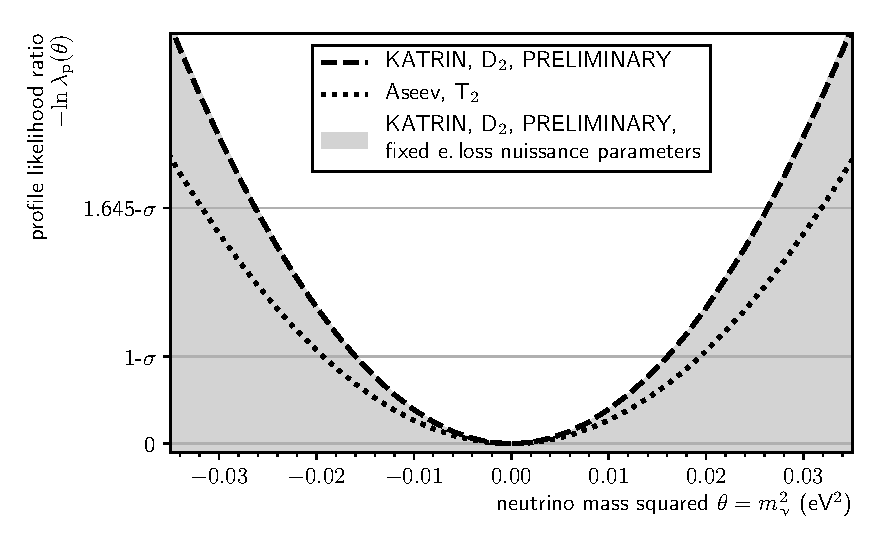
\includegraphics[width=\textwidth]{\currentFigureFolder/profileLikelihoodKATRINandAseev.pdf}
	\xcaption{}{}{}
	\label{fig:katrinElossResultsProfileLikelihood}
\end{figure}

\begin{figure}[th]
	\centering
	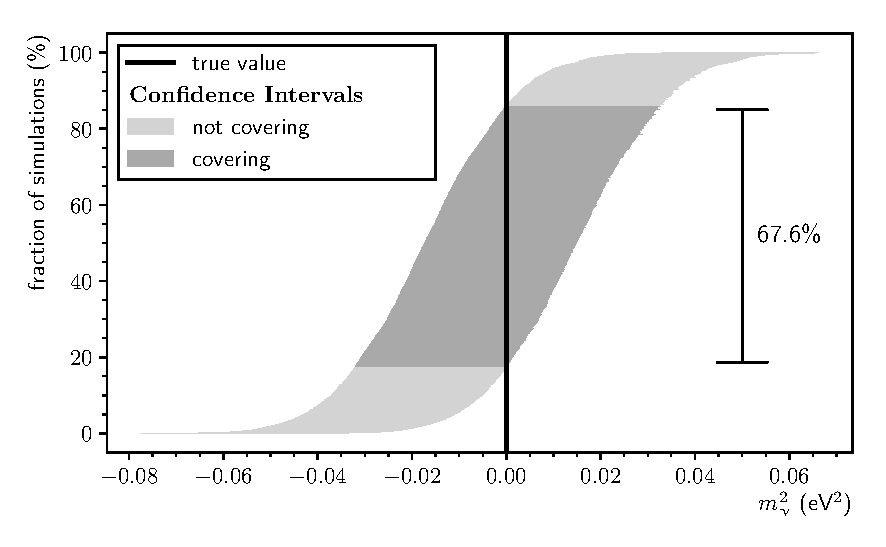
\includegraphics[width=\textwidth]{\currentFigureFolder/coverage.pdf}
	\xcaption{Coverage Test for confidence interval}{}{}
	\label{fig:katrinElossResultsCoverage}
\end{figure}


\section{Conclusion and Outlook}
\label{sec:katrinElossModelConclusion}